\documentclass{article}
\usepackage{graphicx}
\usepackage{amsmath}
\usepackage{natbib}
\usepackage{xcolor}
\usepackage{amssymb}
\newtheorem{proof}{Proof}
\newtheorem{lemma}{Lemma}
\usepackage[margin=1in]{geometry}

\begin{document}


\title{Sequential Cognition Processes: A Framework For Reasoning with Non-Monotonic Logics}
\author{Axel Ind \\ axeltind@gmail.com \\ University of Freiburg}

\maketitle

\section{Overview}
For my Master's thesis I intend to describe, implement, and test a novel framework for modelling human reasoners called the Sequential Cognitive Process. SCPs retain most of the expressiveness of the hitherto \textit{ad hoc} approaches to modelling reasoners with non-monotonic logics, but also introduce a number of desirable properties:
\begin{enumerate}
\item They enable modelling of individual reasoners through addition or subtraction of well-described mental operations. This is in contrast to most non-monotonic logic approaches which can model the general reasoner across a number of cognitive tasks but do not extend well to explaining reasoning that deviates from the norm.
\item They standardise a broad class of non-monotonic logical frameworks so that cognitive comparisons, even across different frameworks are possible, in particular I have given some thought to the use of string-matching algorithms borrowed from the field of bioinformatics (such an extended version of the Needleman Wunsch Aglorithm\cite{needleman1970general}) to comparing WSTs as operation sequences.
\item Because they are sequential (essentially linked lists of mental operations) they lend themselves well to traditional search techniques, and their utility in finding -- though not yet justifying -- models of the Suppression Task has already been demonstrated for both general and individual reasoners.
\item They standardise a set of well-founded cognitive processes (such as, the Suppression Effect, Affirmation of the Antecedent, Conjunction Fallacy bias, and the introduction of abnormalities) as reusable epistemic operations which can be constrained or expanded according the needs of the researcher.
\item Because they are sequential sequences of actions, there is certainly potential for traditional heuristic approaches to problem solving.
\end{enumerate}

An existing implementation of this system has already been implemented\footnote{Available on Github: https://github.com/AxelInd/SequentialCognitionPrcoesses. For access, please contact me with your details.} with a focus on the Weak Completion Semantics \citep{holldobler2015weak}. This implementation has proved effective at modelling both the \citep{byrne1989suppressing} and the Wason Selection Task \citep{wason1968reasoning}, with work to expand the implementation ongoing.

\section{What is an SCP}

An SCP is a model of a reasoner, whether individuals or a group. The SCP assumes that some epistemic state (of whatever form the nonmonotonic logic requires) is modified by mental operations in the SCP to reach a final epistemic state that satisfies some goal properties. An SCP Problem $\pi=(s_i,\gamma,M)$ describes the requirements and limitation of the SCP before it is created\footnote{This formulation is inspired by the field of AI Planning}. $s_i$ contains the initial state of the SCP, and $\gamma$ is the goal of the SCP (e.g. to mimic the classical case of the Suppression Task), $M$ is the set of allowable cognitive operations.

The SCP framework makes several core assumptions about the nature of cognition:


\begin{enumerate}
\item Evolving Epistemic States: SCPs are built on the idea that some mental model of the world exists before the problem-solving begins (even if the model is empty), and is updated by each mental process that acts on it, yielding a new epistemic state as output from mental process $m_n$ to be used as input for mental process $m_{n-1}$.
\item Sequential Reasoning: the assumption that a reasoner will perform only one mental operation at a time before moving on to the next one. Although it initially seems very limitting, the complexity of mental operations is unconstrained, and could itself involve parallel processes provided that a unified mental state is achieved before the next operation begins.
\item Reusable Operations: in order to be more than just a container for some other non-monotonic logic, cognitive tasks must share at least some complex operations. If this were not the case, standardising a set of cognitive operations to model unseen tasks would be impossible. Fortunately, there is ample evidence of consistent mental approaches to reasoning \citep{ragni2017formal}.
\item Limited mental processing power: SCPs assume a sequential and finite number of mental operations to reach a goal. Without this property, it would be impossible to accurately model human cognition. Further, there would be no reasonable scoring system for determining the best explanation when multiple SCPs all model the same thought process (the simplest scoring system intuitively simply being the length of the two SCPs and preferring the smaller).
\end{enumerate}

\begin{figure}
\begin{center}
 \centering 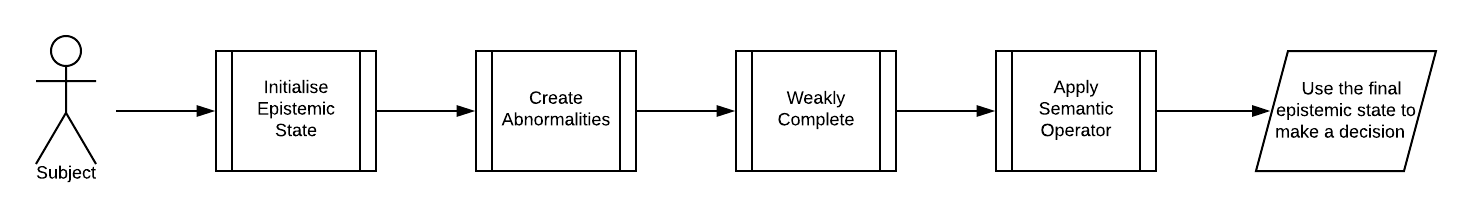
\includegraphics[scale=0.65]{suppressionSCP_overview}
\caption{A generalised illustration of the WCS in an SCP. }
\label {fig:supoverview}
\end{center}
\end{figure}

\begin{figure}
\begin{center}
 \centering 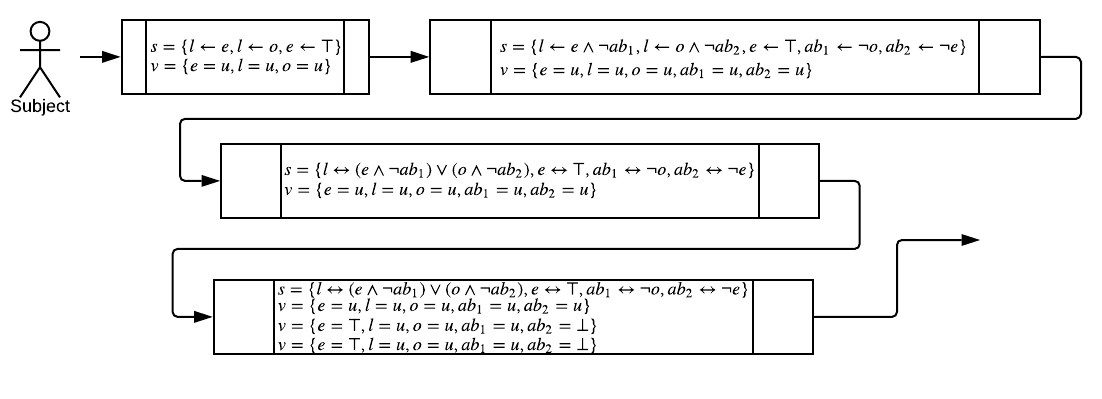
\includegraphics[scale=0.75]{suppressionSCP_normal}
\caption{The standard case of the Suppression Task, demonstrating the suppression effect. }
\label {fig:supnormal}
\end{center}
\end{figure}

For example in its simplest form the Suppression Task with the Suppression Effect modelled under the Weak Completion Semantics could be described in the abstract by Figure~\ref{fig:supoverview} and in terms the epistemic state (containing a set of rules and a set of variables for the Weak Completion Semantics) in Figure~\ref{fig:supnormal}.

\section{Milestones}
A portion of the work to create and formalise SCPs has already been completed. A literature review, time spent programming, and time spent formalising the idea of SCPs has already devoted to the problem. however there is still a significant amount of work to be done:

\subsubsection*{Timeline}
\begin{itemize}
\item Standardise implementation interface: 3 Feb - 9 Feb
\item Extend Interface to Conjunction Fallacy under SCP: 10 Feb - 16 Feb
\item Complete paper on SCPs under the WCS: 17 Feb - 23 Feb
\item Conceptually extend SCPs to Reiter's Default Logic: 24 Feb - 1 March
\item Extend the existing implementation to handle Default Logic: 2 March - 8 March
\item Explore scoring algorithms for SCps: 3 March - 9 March
\item Examine application of heuristics to SCPs: 10 March - 15 March
\item Complete paper on SCPs under Default Logic: 16 March - 23 March
\item Write Thesis: 23 March - 20 April
\item Correction, updates, and new ideas: 21 April - ...
\end{itemize}

\subsubsection*{Deliverables}
\begin{itemize}
\item Conference ready paper on SCPs and the WCS: 23 Feb
\item Conference ready paper on SCPs and the default logic: 23 March
\item Complete, documented, extensible implementation of SCPs containing various examples, search functionality, and best-practice design: 1 April
\end{itemize}
	
\bibliography{bibl}
\bibliographystyle{chicago}









\end{document}
